% Spearman médio com IC 95% por preditor, em ordem decrescente (dados da Tabela tab:res-nivel-feature)
% Cores usadas nesta figura (valores CMYK da paleta dvipsnames do xcolor), definidas aqui para não depender de opções externas
\definecolor{RoyalBlue}{cmyk}{1,0.50,0,0}
\definecolor{BurntOrange}{cmyk}{0,0.51,1,0}
\begin{figure}[htbp]
    \centering
    \caption{Correlação de Spearman média entre a ordenação prevista e a real das \textit{features}, com intervalo de
        confiança de 95\%.}
    \label{fig:res-spearman-ic}
    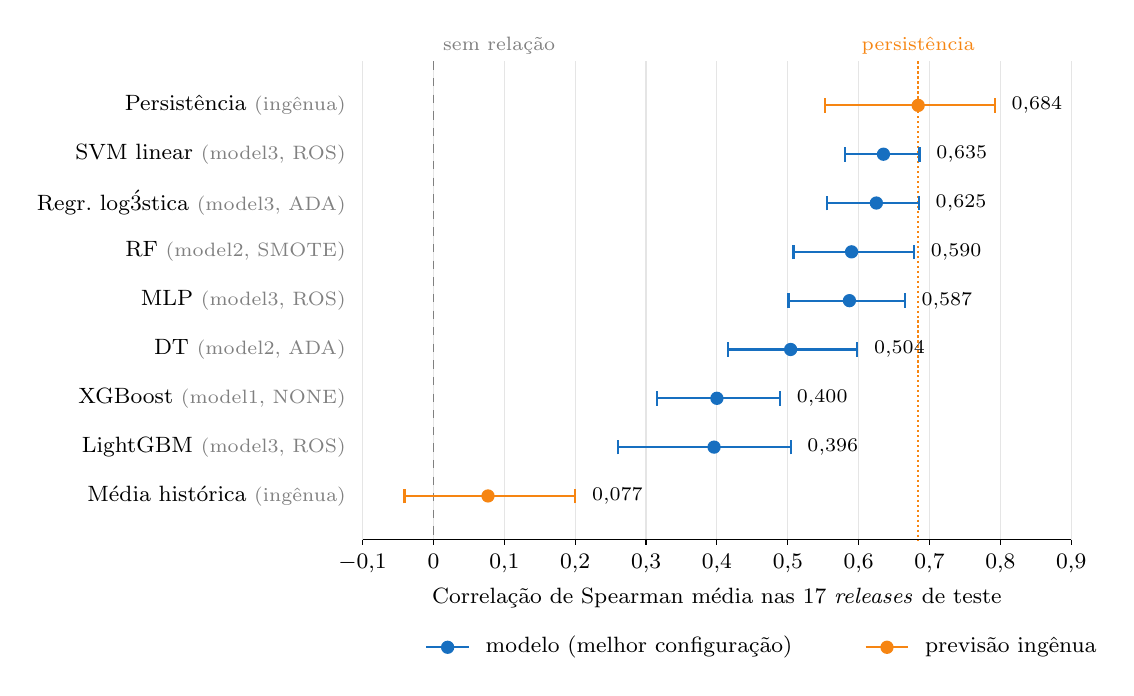
\begin{tikzpicture}[x=9cm,y=0.62cm,font=\footnotesize]
        % eixo x: de -0,1 a 1,0 (1 unidade = 9 cm); linhas de cima para baixo
        \def\xmin{-0.1}
        \def\xmax{0.9}
        % ---- grade e eixo
        \foreach \v/\t in {-0.1/{$-$0{,}1},0/{0},0.1/{0{,}1},0.2/{0{,}2},0.3/{0{,}3},0.4/{0{,}4},0.5/{0{,}5},
                0.6/{0{,}6},0.7/{0{,}7},0.8/{0{,}8},0.9/{0{,}9}}{
            \draw[gray!20] (\v,0.4) -- (\v,-9.4);
            \draw (\v,-9.4) -- (\v,-9.5) node[below] {\t};}
        \draw (\xmin,-9.4) -- (\xmax,-9.4);
        \node[below=14pt] at ({(\xmin+\xmax)/2},-9.4) {Correlação de Spearman média nas 17 \textit{releases} de teste};
        \draw[dashed,gray] (0,0.4) -- (0,-9.4);
        \node[gray,anchor=south west,font=\scriptsize] at (0,0.35) {sem relação};
        \draw[densely dotted,BurntOrange,thick] (0.684,0.4) -- (0.684,-9.4);
        \node[BurntOrange,anchor=south,font=\scriptsize] at (0.684,0.35) {persistência};
        % ---- preditores (nome, configuração, média, IC inferior, IC superior, tipo)
        \foreach \n/\c/\m/\lo/\hi/\tipo [count=\i] in {
                Persistência/ingênua/0.684/0.552/0.792/1,
                SVM linear/{model3, ROS}/0.635/0.581/0.686/0,
                Regr.\ logística/{model3, ADA}/0.625/0.555/0.685/0,
                RF/{model2, SMOTE}/0.590/0.508/0.678/0,
                MLP/{model3, ROS}/0.587/0.501/0.665/0,
                DT/{model2, ADA}/0.504/0.416/0.598/0,
                XGBoost/{model1, NONE}/0.400/0.316/0.489/0,
                LightGBM/{model3, ROS}/0.396/0.260/0.504/0,
                Média histórica/ingênua/0.077/-0.041/0.200/1}{
            \ifnum\tipo=1 \def\cor{BurntOrange}\else \def\cor{RoyalBlue}\fi
            \node[anchor=east] at (\xmin-0.01,-\i+0.5) {\n\ {\scriptsize\color{gray}(\c)}};
            \draw[\cor,thick] (\lo,-\i+0.5) -- (\hi,-\i+0.5);
            \draw[\cor,thick] (\lo,-\i+0.35) -- (\lo,-\i+0.65);
            \draw[\cor,thick] (\hi,-\i+0.35) -- (\hi,-\i+0.65);
            \fill[\cor] (\m,-\i+0.5) circle (2.4pt);
            \pgfmathsetmacro{\lab}{\m}
            \node[anchor=west,font=\scriptsize] at (\hi+0.01,-\i+0.5)
                {\pgfmathprintnumber[fixed,precision=3,fixed zerofill,use comma]{\m}};}
        % ---- legenda
        \begin{scope}[shift={(0.02,-11.6)}]
            \fill[RoyalBlue] (0,0) circle (2.4pt);
            \draw[RoyalBlue,thick] (-0.03,0) -- (0.03,0);
            \node[anchor=west] at (0.04,0) {modelo (melhor configuração)};
            \fill[BurntOrange] (0.62,0) circle (2.4pt);
            \draw[BurntOrange,thick] (0.59,0) -- (0.65,0);
            \node[anchor=west] at (0.66,0) {previsão ingênua};
        \end{scope}
    \end{tikzpicture}
    \fonte{Elaborado pelo autor (2026)}
\end{figure}%
